\documentclass[a4paper,12pt]{article}

% Pacotes úteis
\usepackage[utf8]{inputenc}       % Codificação UTF-8
\usepackage[T1]{fontenc}          % Suporte para acentuação
\usepackage{lmodern}              % Fonte moderna
\usepackage{graphicx}             % Para inclusão de imagens
\usepackage{amsmath}              % Pacote de matemática
\usepackage{amssymb}              % Símbolos matemáticos
\usepackage{geometry}             % Controle das margens
\usepackage{setspace}             % Controle de espaçamento
\usepackage{indentfirst}          % Indentar primeiro parágrafo de cada seção
\usepackage{hyperref}             % Links clicáveis
\usepackage{float}                % Controle de posição de elementos flutuantes (figuras, tabelas)
\usepackage{titlesec}             % Personalização de títulos
         % Para imagens (caso use)
\usepackage{xcolor}           % Para cores nos textos (opcional)
\usepackage{listings}         % Para código C++ (se for incluir trechos)




\documentclass{article}
\usepackage{minted}

% Configurações opcionais para personalizar
\setminted{
    breaklines=true,      % Quebra automaticamente linhas longas
    breakanywhere=true,   % Permite quebrar palavras (opcional)
    frame=lines,          % Adiciona linhas ao redor do código
    fontsize=\small,      % Tamanho da fonte
    breaklines=true,
    breaksymbol=,         % Adiciona um símbolo (opcional)
    breakindent=10pt       % Indenta as linhas quebradas
}



% Configurações de página
% \geometry{left=3cm, right=2cm, top=2cm, bottom=2cm}
% \onehalfspacing                      % Espaçamento de 1,5 entre linhas

% % Cabeçalho com título e autores
% \title{Avaliação de LLM's na extração de dados médicos de notas clínicas}
% \author{
%     Ana Júlia Amaro Pereira Rocha \\ 
%     Maria Eduarda Mesquita Magalhães\\ 
%     Mariana Fernandes Rocha \\ 
%     Paula Eduarda de Lima \\
%     \\ Orientador: Walter Sande
% }
% \date{\today}                         % Data do relatório

% \begin{document}

% \documentclass[12pt,a4paper]{report}
\usepackage{graphicx}
\usepackage{titling}

\documentclass[a4paper,12pt]{article}

\usepackage[portuguese]{babel} % Ativa o português para hifenização
\usepackage[utf8]{inputenc}    % Suporte a caracteres acentuados
\usepackage[T1]{fontenc}       % Fonte com suporte a caracteres especiais
\usepackage{xcolor}
\usepackage[ colorlinks=true, linkcolor=blue,     urlcolor=blue,  citecolor=blue ]{hyperref}
\begin{document}

\begin{titlepage}
    \begin{center}

        \vspace{1cm}
        \begin{minipage}{0.45\textwidth}
            \centering
            
\includegraphics[width=1.2\textwidth]{logo_fgv.png}    
        \end{minipage}
        \vspace{2cm}

        \rule{1\textwidth}{0.4pt} \\ % Linha horizontal personalizada
        \vspace{0.3cm}
        {\Huge \textbf{Pipeline escalável para processamento de dados}} \\
        \vspace{0.2cm}
        \vspace{0.5cm}\\
        {\Large \textbf{A2 Computação Escalável}}\\
        \rule{1\textwidth}{0.4pt} % Linha horizontal personalizada


        \vspace{0.5cm}
        {\Large \textbf{FGV EMAp}} \\
        \vspace{2cm}
        
        

        
        
        % % Unidade e curso
        % {\Large \textbf{FGV EMAp}}\\[2cm]
        
        % Autores
        {\large 
            \textbf{Ana Júlia Amaro Pereira Rocha} \\ 
            \textbf{Henrique Borges Carvalho} \\
            \textbf{Maria Eduarda Mesquita Magalhães}\\
            \textbf{Mariana Fernandes Rocha} \\
            \textbf{Paula Eduarda de Lima}}\\[1.5cm]
        
        % Informações adicionais
        {\large 
            Ciência de Dados e Inteligência Artificial \\ 
            5º Período}\\[2cm]
        
         % Data
        \vfill
        {\large Rio de Janeiro, 2025}

        
    \end{center}
\end{titlepage}

\tableofcontents
\newpage


\section{Introdução}

Este relatório detalha o desenvolvimento de um pipeline escalável para processamento de dados,
conforme proposto no Trabalho 2 da disciplina de Computação Escalável. O objetivo principal é 
evoluir o projeto desenvolvido no Trabalho 1, transformando-o em uma solução distribuída 
capaz de aumentar significativamente sua capacidade de escala. Para atingir este fim, a arquitetura 
da solução foi redefinida, aplicando padrões arquiteturais e tecnologias apresentadas em aula, visando eficiência e escalabilidade.

A solução será implantada em um ambiente de nuvem, especificamente na Amazon Web Services (AWS),
embora seja projetada para também ser executada em uma única máquina para fins de desenvolvimento. 
Este documento abordará a modelagem da arquitetura e do banco de dados, as principais
decisões de projeto, e a apresentação e discussão dos resultados experimentais obtidos.

\section{Modelagem}

Este projeto implementa uma pipeline de processamento de dados distribuída e modular, baseada em \textbf{Apache Kafka}, \textbf{Apache Spark} (nos tratadores), e containers \textbf{Docker} para orquestração dos serviços. Quando executado localmente, todo o ambiente é gerenciado por Docker, garantindo isolamento, reprodutibilidade e facilidade de implantação.

\subsection{Arquitetura Geral}

O ambiente é definido via \texttt{docker-compose.yml}, que orquestra múltiplos containers divididos em três categorias principais:

\begin{itemize}
  \item \textbf{Serviços de infraestrutura e mensageria}: 
          \begin{itemize}
          \item \textbf{Zookeeper}: Gerencia a coordenação dos brokers Kafka.
          \item \textbf{Kafka}: Middleware de mensageria baseado em tópicos.
          \end{itemize}
  \item \textbf{Geradores e tratadores de dados}:
  \begin{itemize}
  \item \textbf{mock-generator}: Gera dados sintéticos e os envia ao Kafka.
  \item \textbf{tratador-limpeza}: Realiza a limpeza inicial dos dados.
  \item \textbf{tratador-filtragem}: Aplica filtros aos dados limpos e publica em novos tópicos.
  \item \textbf{tratador-media}: Focado em médias por região.
  \item \textbf{tratador-merge}: Responsável por unificar dados vindos de diferentes tratadores em um único artefato de saída.
    \item \textbf{tratador-agrupar-colunas}: Agrupar variáveis relacionadas e criar estruturas auxiliares para análise estatística posterior.
    \item \textbf{tratador-correlacao}: Calcular correlação entre variáveis (ex: vacinação vs. número de casos).
    \item \textbf{tratador-desvio-padrao}: Avaliar a variabilidade dos dados, detectar instabilidades e anomalias.
    \item \textbf{tratador-mediamovel}: Aplicar suavização dos dados no tempo, útil para observar tendências (ex: 7 dias, 14 dias).
    \item \textbf{tratador-regressao}: Aplicar modelos estatísticos para prever variáveis (ex: número de casos futuros).
\end{itemize}
    \item Serviços de Interface 

    \begin{itemize}
  \item \textbf{API (FastAPI):} fornece uma interface REST para acesso aos dados processados.
  \item \textbf{Dashboard (Streamlit):} apresenta os resultados de forma visual e interativa.
\end{itemize}
\end{itemize}

\subsection{Resumo}

\begin{itemize}
  \item A arquitetura segue o padrão \textbf{event-driven}, com os tratadores consumindo e publicando dados via Kafka.
  \item O uso de \textbf{volumes persistentes} permite manter os dados entre execuções e facilita o rastreamento de artefatos.
  \item A divisão modular permite escalar tratadores de forma independente.
  \item \textbf{O ambiente local é executado inteiramente em containers Docker}, permitindo desenvolvimento e testes isolados.
\end{itemize}

\section{Mock}

O script \texttt{generator.py} é responsável por simular dados verossímeis de três fontes distintas: Organização Mundial da Saúde (OMS), hospitais e Secretaria de Saúde (SS). Cada fonte envia mensagens JSON para um tópico Kafka específico (\texttt{raw\_oms}, \texttt{raw\_hospital}, \texttt{raw\_secretary}) com dados fictícios representando registros semanais.

A estrutura geográfica utilizada define 20 ``ilhas'', identificadas por CEPs de dois dígitos (de 11 a 30), cada uma subdividida em 5 ``regiões'' com CEPs de cinco dígitos (por exemplo, ilha 12 $\rightarrow$ CEPs 12001 a 12005). As mensagens incluem dados populacionais, diagnósticos, vacinação, sintomas, escolaridade, entre outros. As datas dos registros são aleatórias, mas sempre dentro da semana corrente, simulando atualizações semanais realistas.

O script opera em ciclos controlados por uma variável de ambiente (INTERVALO\_CICLO) e permite configurar o número de registros gerados por ciclo. Além de enviar os dados para o Kafka. Esse mock automatizado viabiliza testes realistas do pipeline de processamento com dados heterogêneos e estruturados.

Para cada fonte, são gerados atributos coerentes e controlados para manter a verossimilhança dos dados. Por exemplo, o número de vacinados nunca excede o valor da população, e os sintomas hospitalares são combinados com informações como idade, sexo e internação. 

Além disso, as variáveis são simuladas de forma a refletir correlações plausíveis entre escolaridade, vacinação e diagnósticos, permitindo análises estatísticas significativas nos módulos de tratamento e visualização.


\vspace{0.5cm}

\textbf{Fontes e dados gerados}

\begin{itemize}
    \item \textcolor{purple}{\textbf{OMS}}\\
    Dados agregados por ilha (CEP de 2 dígitos).\\
    Inclui número de óbitos, população, recuperados, vacinados e data.
    
    \vspace{0.5em}
    
    \item \textcolor{red}{\textbf{Hospitais }}\\
    Dados individuais por paciente, com CEPs de 5 dígitos (regiões).\\
    Contém informações como internação, idade, sexo, sintomas e data.
    
    \vspace{0.5em}
    
    \item \textcolor{orange}{\textbf{Secretaria de Saúde}}\\
    Dados por região (CEP de 5 dígitos): diagnóstico, vacinação, escolaridade, população e data..
\end{itemize}


\section{Tratadores}

O sistema conta com diversos tratadores Spark responsáveis por consumir os dados brutos ou parcialmente processados a partir de tópicos Kafka, aplicar transformações específicas e enviar resultados para tópicos subsequentes ou APIs intermediárias. A seguir, descrevemos o papel de cada tratador utilizado na arquitetura.

\subsection{Tratador 1: Limpeza}

Este módulo é responsável por realizar a limpeza inicial dos dados oriundos das três fontes (OMS, hospitais e secretaria). 

Ele consome registros dos tópicos Kafka \texttt{raw\_secretary}, \texttt{raw\_hospital} e \texttt{raw\_oms}, e aplica filtros estruturais e semânticos utilizando Apache Spark.

O esquema esperado é rigorosamente definido com seis campos: diagnóstico, vacinação, CEP (região), escolaridade, população e data. Para garantir a qualidade dos dados, o tratador executa filtros que eliminam registros inconsistentes, incluindo:
\begin{itemize}
    \item valores de \texttt{Diagnostico} e \texttt{Vacinado} fora do domínio binário (0 ou 1);
    \item \texttt{Escolaridade} fora do intervalo de 0 a 5;
    \item \texttt{CEP}s inválidos (fora do intervalo 11001--30999);
    \item \texttt{População} menor ou igual a zero;
    \item \texttt{Data} nula.
\end{itemize}

Os dados são processados em lotes (\textit{batches}) de n registros. Cada lote é transformado em um DataFrame Spark, filtrado conforme os critérios acima, e os registros válidos são serializados em JSON e enviados para os tópicos seguinte do pipeline,  \texttt{clean\_secretary} \texttt{clean\_hospital} e \texttt{clean\_oms}. Esse processamento por lote permite balancear desempenho com controle de qualidade e manter o paralelismo nativo do Spark.

% Embora o Redis esteja previsto na arquitetura geral como armazenamento auxiliar, este tratador em específico não realiza operações diretas sobre ele. Seu foco é assegurar que apenas dados limpos sigam adiante para tratadores analíticos posteriores.



\subsection{Tratador 2: Filtragem}

Este módulo é responsável pela filtragem contínua dos dados previamente limpos, operando em modo \textit{streaming} com Apache Spark. Ele consome dados dos respectivos tópicos, por exemplo \texttt{clean\_secretary}, realizando validações adicionais para garantir que apenas registros relevantes e consistentes avancem no pipeline.

A filtragem aplicada segue os seguintes critérios:
\begin{itemize}
    \item \texttt{População} superior a 500, descartando regiões com baixa significância estatística;
    \item presença obrigatória não nula dos campos \texttt{Número de Óbitos} e/ou \texttt{Número de Recuperados} na fonte OMS;
    \item Verifica a coluna idade esta no intervalo de $$[0,120]$
    \item o registro deve conter pelo menos um evento relevante, ou seja, estar vacinado (\texttt{Vacinado} = 1) ou ter recebido diagnóstico (\texttt{Diagnostico} = 1).
\end{itemize}

A implementação utiliza leitura em fluxo (\texttt{readStream}) diretamente do Kafka, com parsing de mensagens JSON para um DataFrame tipado. Após a aplicação dos filtros, os dados são reserializados em JSON e enviados ao tópico \texttt{filtered\_secretary}, \texttt{filtered\_hospital} e \texttt{filtered\_oms}, que servem como entrada para módulos analíticos subsequentes.

A arquitetura de streaming adotada neste tratador permite que o pipeline processe os dados com baixa latência e alta escalabilidade, mantendo tolerância a falhas via checkpoints no sistema de arquivos. Dessa forma, o tratador garante que somente dados robustos e analiticamente relevantes passem para as próximas etapas, como agregações e inferências estatísticas.


\subsection{Tratador 3: Merge}

O Tratador 3 é responsável por unir dados hospitalares e da secretaria de saúde com base na localização geográfica (\texttt{CEP}), utilizando Apache Spark para agregações eficientes. Seu objetivo é consolidar múltiplas fontes em um único conjunto de dados enriquecido, pronto para análises posteriores.

Este módulo trata dois cenários de forma diferenciada:

\begin{itemize}
    \item \textbf{Dados históricos}: São acumulados em memória até que ambas as fontes indiquem o fim dos envios. Ao receber os sinais de término, o módulo realiza um processamento único e completo do histórico.
    \item \textbf{Dados normais}: Lotes são processados em tempo real assim que ambas as fontes (hospital e secretaria) fornecem registros correspondentes.
\end{itemize}

Os dados são consumidos de dois tópicos Kafka simultaneamente. Cada lote recebido é decodificado e categorizado conforme sua origem e tipo (histórico ou normal). O schema é previamente definido para ambas as fontes, assegurando tipagem explícita dos dados recebidos.

O processamento consiste em:
\begin{enumerate}
    \item Agregar as informações hospitalares por \texttt{CEP}, somando variáveis como número de internados presença de sintomas.
    \item Agregar os dados da secretaria por \texttt{CEP}, computando totais de diagnósticos, vacinados, média de escolaridade e idade dos pacientes.
    \item Unir os dois conjuntos agregados com uma junção externa (\texttt{outer join}), preservando todos os \texttt{CEPs} mesmo quando presentes apenas em uma das fontes.
\end{enumerate}

Esse modelo híbrido de ingestão torna o pipeline flexível, permitindo tanto reprocessamentos históricos quanto ingestão contínua em tempo real, com baixa latência e alta escalabilidade. O resultado é um DataFrame Spark unificado por região, apto para alimentar tratadores analíticos subsequentes.



\subsection{Tratador 4: Agrupamento por Colunas}

O quarto tratador realiza o agrupamento estatístico dos dados filtrados, consolidando métricas por região geográfica (\texttt{CEP}). Este agrupamento é executado em lote com Apache Spark, preservando o paralelismo e escalabilidade do processamento.

A cada lote de mensagens Kafka recebidas dos tópicos \texttt{filtered\_hospital},  \texttt{filtered\_oms} e  \texttt{filtered\_secretary}, os dados são lidos como JSON e convertidos em um \textit{DataFrame} tipado. Em seguida, são agregados com base no campo \texttt{CEP} e \texttt{Data}, produzindo estatísticas como:
\begin{itemize}
    \item soma de diagnósticos positivos (\texttt{Diagnostico});
    \item soma da variável binária de sintoma (\texttt{Sintoma 1,2,3,4});
    \item média de escolaridade (\texttt{Escolaridade});
    \item população declarada da região;
    \item total de vacinados por CEP;
\end{itemize}

O resultado é simultaneamente enviado para dois destinos: o tópico Kafka \texttt{grouped\_secretary}, \texttt{grouped\_hospital} e \texttt{grouped\_oms} que serve de insumo para etapas analíticas posteriores, e uma API REST, que recebe os dados agregados para persistência ou visualização.

A estratégia de processamento por lotes, combinada com o uso de funções de agregação distribuídas, permite a eficiente consolidação de dados em grande escala. Esse tratador é fundamental para reduzir a granularidade da base e extrair conhecimento agregado por unidade territorial, o que é essencial para análises de correlação, regressão e predição.



\subsection{Tratador 5: Média Populacional e Alertas}

O Tratador 5 é responsável por calcular a média do número de óbitos de todas as regiões dos registros recebidos da OMS e gerar alertas com base nessa métrica. Seu principal objetivo é destacar regiões com fatalidade acima da média por meio de marcações automáticas no fluxo de dados.

Este módulo consome mensagens em lote do tópico Kafka \texttt{filtered\_oms}, contendo dados da Organização Mundial da Saúde (OMS), como número de óbitos, recuperados, vacinados e população por \texttt{CEP}. O processamento é feito em modo \textit{batch}, utilizando Apache Spark para tratar e transformar os dados.

O funcionamento do tratador envolve os seguintes passos:
\begin{enumerate}
    \item Conversão do lote Kafka em um \textit{DataFrame} com schema tipado.
    \item Cálculo da média de mortes dos registros do lote.
    \item Classificação de cada linha com base na comparação entre a população local e a média:
        \begin{itemize}
            \item Se óbitos do \texttt{CEP} for maior que a média, o campo \texttt{Alerta} recebe o valor \texttt{Vermelho};
            \item Caso contrário, o alerta é classificado como \texttt{Verde}.
        \end{itemize}
    \item Geração de um arquivo consolidado no formato JSON contendo os dados com o alerta marcado.
\end{enumerate}

O resultado é salvo localmente em \texttt{alerta\_batch.json}, podendo ser utilizado por serviços downstream para fins de monitoramento ou visualização. Além disso, o consumidor Kafka confirma o processamento de cada batch após sua conclusão, garantindo consistência e controle sobre o fluxo de mensagens.

Este tratador oferece uma camada adicional de inteligência ao pipeline, destacando dinamicamente regiões com maior densidade populacional e permitindo respostas mais direcionadas por parte das autoridades de saúde.



\subsection{Tratador 6: Correlação}

Este módulo é responsável por calcular correlações estatísticas entre variáveis de interesse a partir dos dados agregados por CEP. Utilizando a função \texttt{corr} do Spark, ele avalia a dependência linear entre atributos como média de escolaridade e média de vacinação, aproveitando o paralelismo do Spark para garantir desempenho mesmo com grandes volumes de dados.

O processo funciona em modo batch, consumindo dados dos tópicos Kafka \\ \texttt{grouped\_hospital}, \texttt{grouped\_secretary} e \texttt{grouped\_oms}. A cada lote, os dados são convertidos em um DataFrame tipado (com schema explícito), o que assegura integridade e desempenho durante os cálculos estatísticos.

Os resultados das correlações são transformados em JSON e enviados para uma API intermediária responsável por alimentar o dashboard com insights visuais. Embora o código atual esteja configurado para calcular apenas a correlação entre \texttt{media\_escolaridade} e \texttt{total\_vacinado}, a estrutura do módulo é extensível para múltiplas combinações de variáveis no futuro.



\subsection{Tratador 7: Desvio Padrão}

Este módulo é responsável por calcular o desvio padrão de métricas regionais previamente agregadas por CEP, como média de diagnósticos, vacinação, escolaridade e população. O objetivo principal é quantificar a variabilidade estatística entre as regiões, fornecendo indicadores de dispersão que podem revelar comportamentos atípicos ou inconsistentes nos dados.

O tratador opera de forma \textit{batch}, consumindo mensagens do tópico  \\ \texttt{grouped\_secretary}, convertendo-as diretamente em um \textit{DataFrame} com \textit{schema} tipado e realizando as agregações com a função \texttt{stddev()} do Spark. Para manter a performance e escalabilidade, todos os cálculos são distribuídos em paralelo.

Os resultados, formatados em estruturas nomeadas (\texttt{named\_struct}) e reorganizados via \texttt{stack}, são convertidos em JSON e enviados para a API \texttt{/desvios}, que alimenta visualizações no dashboard final. Esse formato permite acompanhar a dispersão estatística de cada variável monitorada, facilitando diagnósticos populacionais e a identificação de regiões fora do padrão. O resultado permite identificar regiões com maior variabilidade e possíveis anomalias.

\subsection{Tratador 8: Regressão e Métricas}

Este tratador realiza a análise estatística contínua dos dados filtrados, calculando métricas agregadas de forma incremental a partir das variáveis \texttt{Vacinado}, \texttt{Escolaridade}, \texttt{Populacao} e \texttt{Diagnostico}. A cada lote de 10 registros recebidos do tópico \texttt{filtered\_secretary}, ele executa uma agregação com Spark utilizando as funções \texttt{mean()} e \texttt{avg()} para gerar indicadores como taxa média de vacinação, escolaridade média, taxa de diagnóstico e média populacional.

Embora o nome do módulo indique "regressão", o código atual não implementa uma regressão linear multivariada explícita, mas sim calcula métricas estatísticas que servem como base para análises interpretáveis posteriores, incluindo visualizações de tendências e preparação de dados para modelos preditivos.

Os resultados são armazenados em um arquivo JSON e enviados periodicamente para uma API REST (\texttt{/metricas}) que alimenta o dashboard. O módulo foi projetado para ser eficiente e robusto, operando de forma contínua e paralelizada com Apache Spark, garantindo escalabilidade mesmo com grandes volumes de dados.


\subsection{Tratador 8: Regressão}

Este módulo executa uma regressão linear multivariada utilizando variáveis como escolaridade, população e vacinação para prever diagnósticos. A inclinação (coeficiente beta) de cada variável é armazenada e exibida no dashboard para análise interpretável.

\subsection{Tratador 9: Média Móvel}

Este tratador é responsável por calcular a média móvel da taxa de diagnósticos ao longo do tempo, com o objetivo de suavizar flutuações diárias e identificar tendências epidemiológicas. Ele consome dados do tópico \texttt{grouped\_secretary}, realiza agregações por data e aplica uma janela deslizante de 7 dias utilizando a API de janelas do Spark (\texttt{Window}).

O campo \texttt{Data}, inicialmente em formato de string (\texttt{dd-MM-yyyy}), é convertido para o tipo de data nativo do Spark para permitir operações temporais. Em seguida, os diagnósticos são agrupados por data e sua média é calculada. Sobre essa série temporal, é aplicada uma janela móvel de 7 dias que gera, para cada dia, a média dos valores nos últimos sete dias (inclusive o atual), produzindo uma curva suavizada de evolução dos casos.

O valor da média móvel para a data mais recente é extraído e enviado para uma API REST (\texttt{/media-movel}) para posterior visualização no dashboard. Este tratador permite, portanto, detectar padrões de crescimento ou queda nos diagnósticos com maior robustez estatística frente a variações esporádicas.

\subsubsection*{Pontos fortes específicos da abordagem}

A arquitetura modular dos tratadores permite escalabilidade, paralelismo e flexibilidade no processamento de dados heterogêneos em diferentes estágios do pipeline. A divisão clara de responsabilidades — como limpeza, filtragem, agregações, cálculos estatísticos e inferência — favorece a manutenção e facilita reprocessamentos ou substituição de módulos de forma isolada. O uso intensivo de Apache Spark, tanto em modo \textit{batch} quanto \textit{streaming}, garante desempenho mesmo com grandes volumes de dados. A padronização da comunicação entre módulos via Kafka possibilita desacoplamento, tolerância a falhas e compatibilidade com arquiteturas distribuídas reais. Além disso, a presença de tratadores analíticos como os de regressão, correlação e média móvel permite que o pipeline vá além da ingestão e se torne uma ferramenta de suporte à decisão baseada em dados.


\subsubsection*{Pontos fracos específicos da abordagem}

Apesar da robustez e escalabilidade, a abordagem adotada apresenta desafios de complexidade operacional. O elevado número de tratadores exige orquestração cuidadosa para garantir a ordem e a integridade no fluxo de dados, aumentando o custo de manutenção e depuração. Além disso, muitos módulos operam de forma independente, o que pode dificultar o rastreamento de erros e o controle de versões intermediárias dos dados. Por fim, embora o Spark ofereça ótimo desempenho, ele requer recursos computacionais elevados, e sua configuração incorreta pode comprometer a performance e gerar latências inesperadas.



\section{Dashboard}

O dashboard foi desenvolvido com a biblioteca Streamlit e tem como objetivo principal a visualização integrada das 10 métricas geradas pelos diferentes tratadores da pipeline de dados. Ele permite acompanhar, de forma interativa e interpretável, indicadores estatísticos de saúde extraídos a partir de dados simulados e processados em tempo real via Kafka e Spark.

O dashboard se conecta a uma API REST  e consulta diversos endpoints correspondentes aos tratadores T4 a T9. A cada execução, os dados retornados são carregados em DataFrames do Pandas e visualizados em forma de tabelas, gráficos de linha, barras e dispersão.


\subsection*{Métricas calculadas mostradas}

\begin{itemize}
    \item \textbf{1. Evolução histórica da taxa de vacinados:} 
    \begin{itemize}
        \item Calculada como \texttt{vacinados / população} ao longo do tempo;
        \item Envolve limpeza dos dados e agregação por data (\texttt{tratador 1}, \texttt{tratador 4}).
    \end{itemize}

    \item \textbf{2. Evolução histórica de diagnosticados:}
    \begin{itemize}
        \item Monitora a quantidade de diagnósticos ao longo do tempo;
        \item Requer limpeza e agrupamento por data (\texttt{tratador 1}, \texttt{tratador 4}).
    \end{itemize}

    \item \textbf{3. Correlação entre escolaridade e vacinação:}
    \begin{itemize}
        \item Avalia a relação linear entre escolaridade média e taxa de vacinação;
        \item Baseia-se em dados limpos e agregados (\texttt{tratador 1}, \texttt{tratador 4}), processados por módulo de correlação (\texttt{tratador 6}).
    \end{itemize}

    \item \textbf{4. Média de diagnosticados:}
    \begin{itemize}
        \item Calcula a média de diagnósticos por lote de dados filtrados;
        \item Executada após limpeza e agregação (\texttt{tratador 1}, \texttt{tratador 8}).
    \end{itemize}

    \item \textbf{5. Correlação entre vacinação e internações:}
    \begin{itemize}
        \item Realizada após mesclagem dos dados da secretaria e hospitais (\texttt{tratador 3});
        \item Utiliza correlação estatística entre variáveis agregadas.
    \end{itemize}

    \item \textbf{6. Estatística descritiva por região:}
    \begin{itemize}
        \item Gera desvio padrão de variáveis como escolaridade, população, vacinação e diagnóstico;
        \item Exige limpeza, merge e cálculo de dispersão (\texttt{tratador 1}, \texttt{tratador 3}, \texttt{tratador 7}).
    \end{itemize}

    \item \textbf{7. Regressão linear para predição de diagnóstico:}
    \begin{itemize}
        \item Regressão multivariada baseada em escolaridade, vacinação e população;
        \item Depende de dados limpos e mesclados (\texttt{tratador 1}, \texttt{tratador 3}, \texttt{tratador 8}).
    \end{itemize}

    \item \textbf{8. Estatísticas hospitalares globais:}
    \begin{itemize}
        \item Cálculo de médias e desvios para sintomas, idade, internações por CEP;
        \item Envolve limpeza, agregação e operações estatísticas (\texttt{tratador 3}).
    \end{itemize}

    \item \textbf{9. Ranking de vacinação por região:}
    \begin{itemize}
        \item Ordena regiões com base na média de vacinação;
        \item Gerado a partir de dados limpos e agregados (\texttt{tratador 4}).
    \end{itemize}

    \item \textbf{10. Predição de tendência via média móvel:}
    \begin{itemize}
        \item Aplica janela temporal sobre séries de diagnósticos diários;
        \item Utiliza agregação por data e média móvel de 7 dias (\texttt{tratador 9}).
    \end{itemize}
\end{itemize}


% \begin{itemize}
% \item \textbf{Métricas Gerais (API /metricas)}: Exibe a evolução de indicadores agregados como taxa de vacinação, escolaridade média, taxa de diagnóstico e população média. Os gráficos associados mostram a variação dessas métricas em função da quantidade de dados acumulados, possibilitando o monitoramento da consistência do sistema ao longo do tempo.
% \item \textbf{Agrupamento por Região (T4)}: Mostra os dados agregados por CEP, permitindo a análise espacial dos diagnósticos. A média de diagnósticos por região é apresentada em um gráfico de barras, o que facilita a identificação de áreas mais afetadas.

% \item \textbf{Correlação Escolaridade/Vacinação (T6)}: Exibe os coeficientes de correlação entre variáveis-chave. Um gráfico de dispersão mostra visualmente a relação linear entre escolaridade média e taxa de vacinação, evidenciando padrões de associação que podem ser explorados para análise causal.

% \item \textbf{Desvios Padrão por Região (T7)}: Mostra o grau de variabilidade das variáveis agregadas. O gráfico de barras evidencia quais variáveis possuem maior dispersão entre as regiões, podendo indicar desigualdade territorial ou anomalias nos dados.

% \item \textbf{Regressão Linear Multivariada (T8)}: Apresenta os coeficientes (\textit{betas}) obtidos a partir de uma regressão linear multivariada com as variáveis independentes (vacinação, escolaridade e população) utilizadas para prever diagnósticos. Os betas são visualizados em um gráfico de barras, indicando a força e direção da influência de cada variável.

% \item \textbf{Média Móvel de Diagnósticos (T9)}: Mostra a tendência temporal dos diagnósticos por meio de uma média móvel de 7 dias. O gráfico de linha evidencia momentos de crescimento ou redução no número de casos, permitindo uma visão suavizada das flutuações diárias.

% \end{itemize}

A atualização de todos os dados é em tempo real. O cache automático é invalidado a cada 60 segundos para evitar sobrecarga desnecessária na API, mantendo o desempenho do sistema.


ADICIONAR FOTO DO DASHBOARD


\section{Ambiente Docker}

O ambiente do sistema é orquestrado com \textit{Docker Compose} na versão 3.9, que define os serviços necessários para o funcionamento completo do pipeline de dados, análises e visualização.


\begin{itemize}
    \item Todos os serviços configuram políticas de reinício automático (\texttt{restart: unless-stopped}), garantindo alta disponibilidade.
    \item Os serviços dependem uns dos outros via \texttt{depends\_on} com checagem de saúde, garantindo a ordem correta de inicialização.
    \item Volumes nomeados são utilizados para persistência dos dados de Zookeeper, Kafka.
\end{itemize}

Essa arquitetura baseada em containers facilita a implantação, escalabilidade e manutenção do pipeline completo, permitindo replicação consistente do ambiente em diferentes máquinas ou clusters.


\section{Ambiente Nuvem - AWS}

Para a implementação em nuvem, utilizamos serviços da Amazon AWS fornecidos pela conta \textit{AWS Academy}. Algumas escolhas de serviços e soluções adotadas decorreram das limitações dessa conta, como permissões e restrições de serviços disponíveis. Outras decisões foram motivadas pela própria arquitetura do pipeline.

Nossa arquitetura em nuvem busca ser o mais semelhante possível ao ambiente local, tanto por razões arquiteturais quanto por razões de negócio. Do ponto de vista de negócios, é vantajoso que o ambiente de produção na nuvem se assemelhe ao ambiente local, pois isso facilita a realização de testes, otimizações e mudanças no projeto localmente, sem grandes esforços para replicá-las na nuvem.

Foram utilizados os serviços \textbf{ECS}, \textbf{ECR} e \textbf{EC2} para a implementação em nuvem. A estrutura da aplicação utiliza uma estratégia de \textit{pub/sub}, e, do ponto de vista dos tratadores, essa abordagem se assemelha a uma arquitetura de microserviços, o que justifica a arquitetura proposta.

\subsection{Gerador de Dados}

Para o gerador de dados, foi utilizado um serviço do \textbf{ECS}, o que permite controlar a quantidade de produtores e realizar testes de carga. O gerador de dados possui um \textit{cluster} próprio, no qual foi definido um serviço responsável pela geração dos dados.

O gerador envia dados diretamente para o \textit{broker Kafka}. Idealmente, utilizaríamos o serviço \textbf{Amazon Managed Streaming for Apache Kafka (Amazon MSK)}. No entanto, esse serviço está indisponível na versão de aluno da conta. Como alternativa, o \textbf{Kafka} foi implementado em uma instância \textbf{EC2}. Ressaltamos que não utilizamos o Kafka em um ECS com instância EC2 devido à ausência da permissão \texttt{AmazonEC2ContainerServiceforEC2Role} na conta. Para evitar problemas com endereçamento IP ao alternar sessões, configuramos um \textbf{Elastic IP}.

\subsection{Tratadores}

Para os tratadores, foram criadas diversas \textbf{Task Definitions}, uma para cada tratador, onde configuramos os recursos computacionais (CPU e memória) conforme a carga de processamento esperada. Por exemplo, os tratadores de limpeza e filtragem, localizados no início da pipeline e que processam grandes volumes de dados, receberam mais recursos. Em contrapartida, tratadores com menor volume de dados receberam menos recursos.

\subsection{API e Dashboard}

A \textbf{API} e o \textbf{Dashboard} também foram executados via ECS. No entanto, não foi configurado um \textbf{Elastic IP} para esses serviços, o que aumenta a complexidade, pois o ECS gera IPs dinâmicos. Melhorias futuras podem incluir o uso de ferramentas como:

\begin{itemize}
    \item \textbf{Application Load Balancer (ALB)}
    \item \textbf{Network Load Balancer (NLB)} com IP Elástico
    \item \textbf{AWS PrivateLink}
    \item \textbf{NAT Gateway} com IP Elástico
\end{itemize}

A escolha entre essas soluções depende do objetivo desejado (alta disponibilidade, segurança, desempenho, etc.).


\section{Pipeline}

\begin{figure}[H]
    \centering
    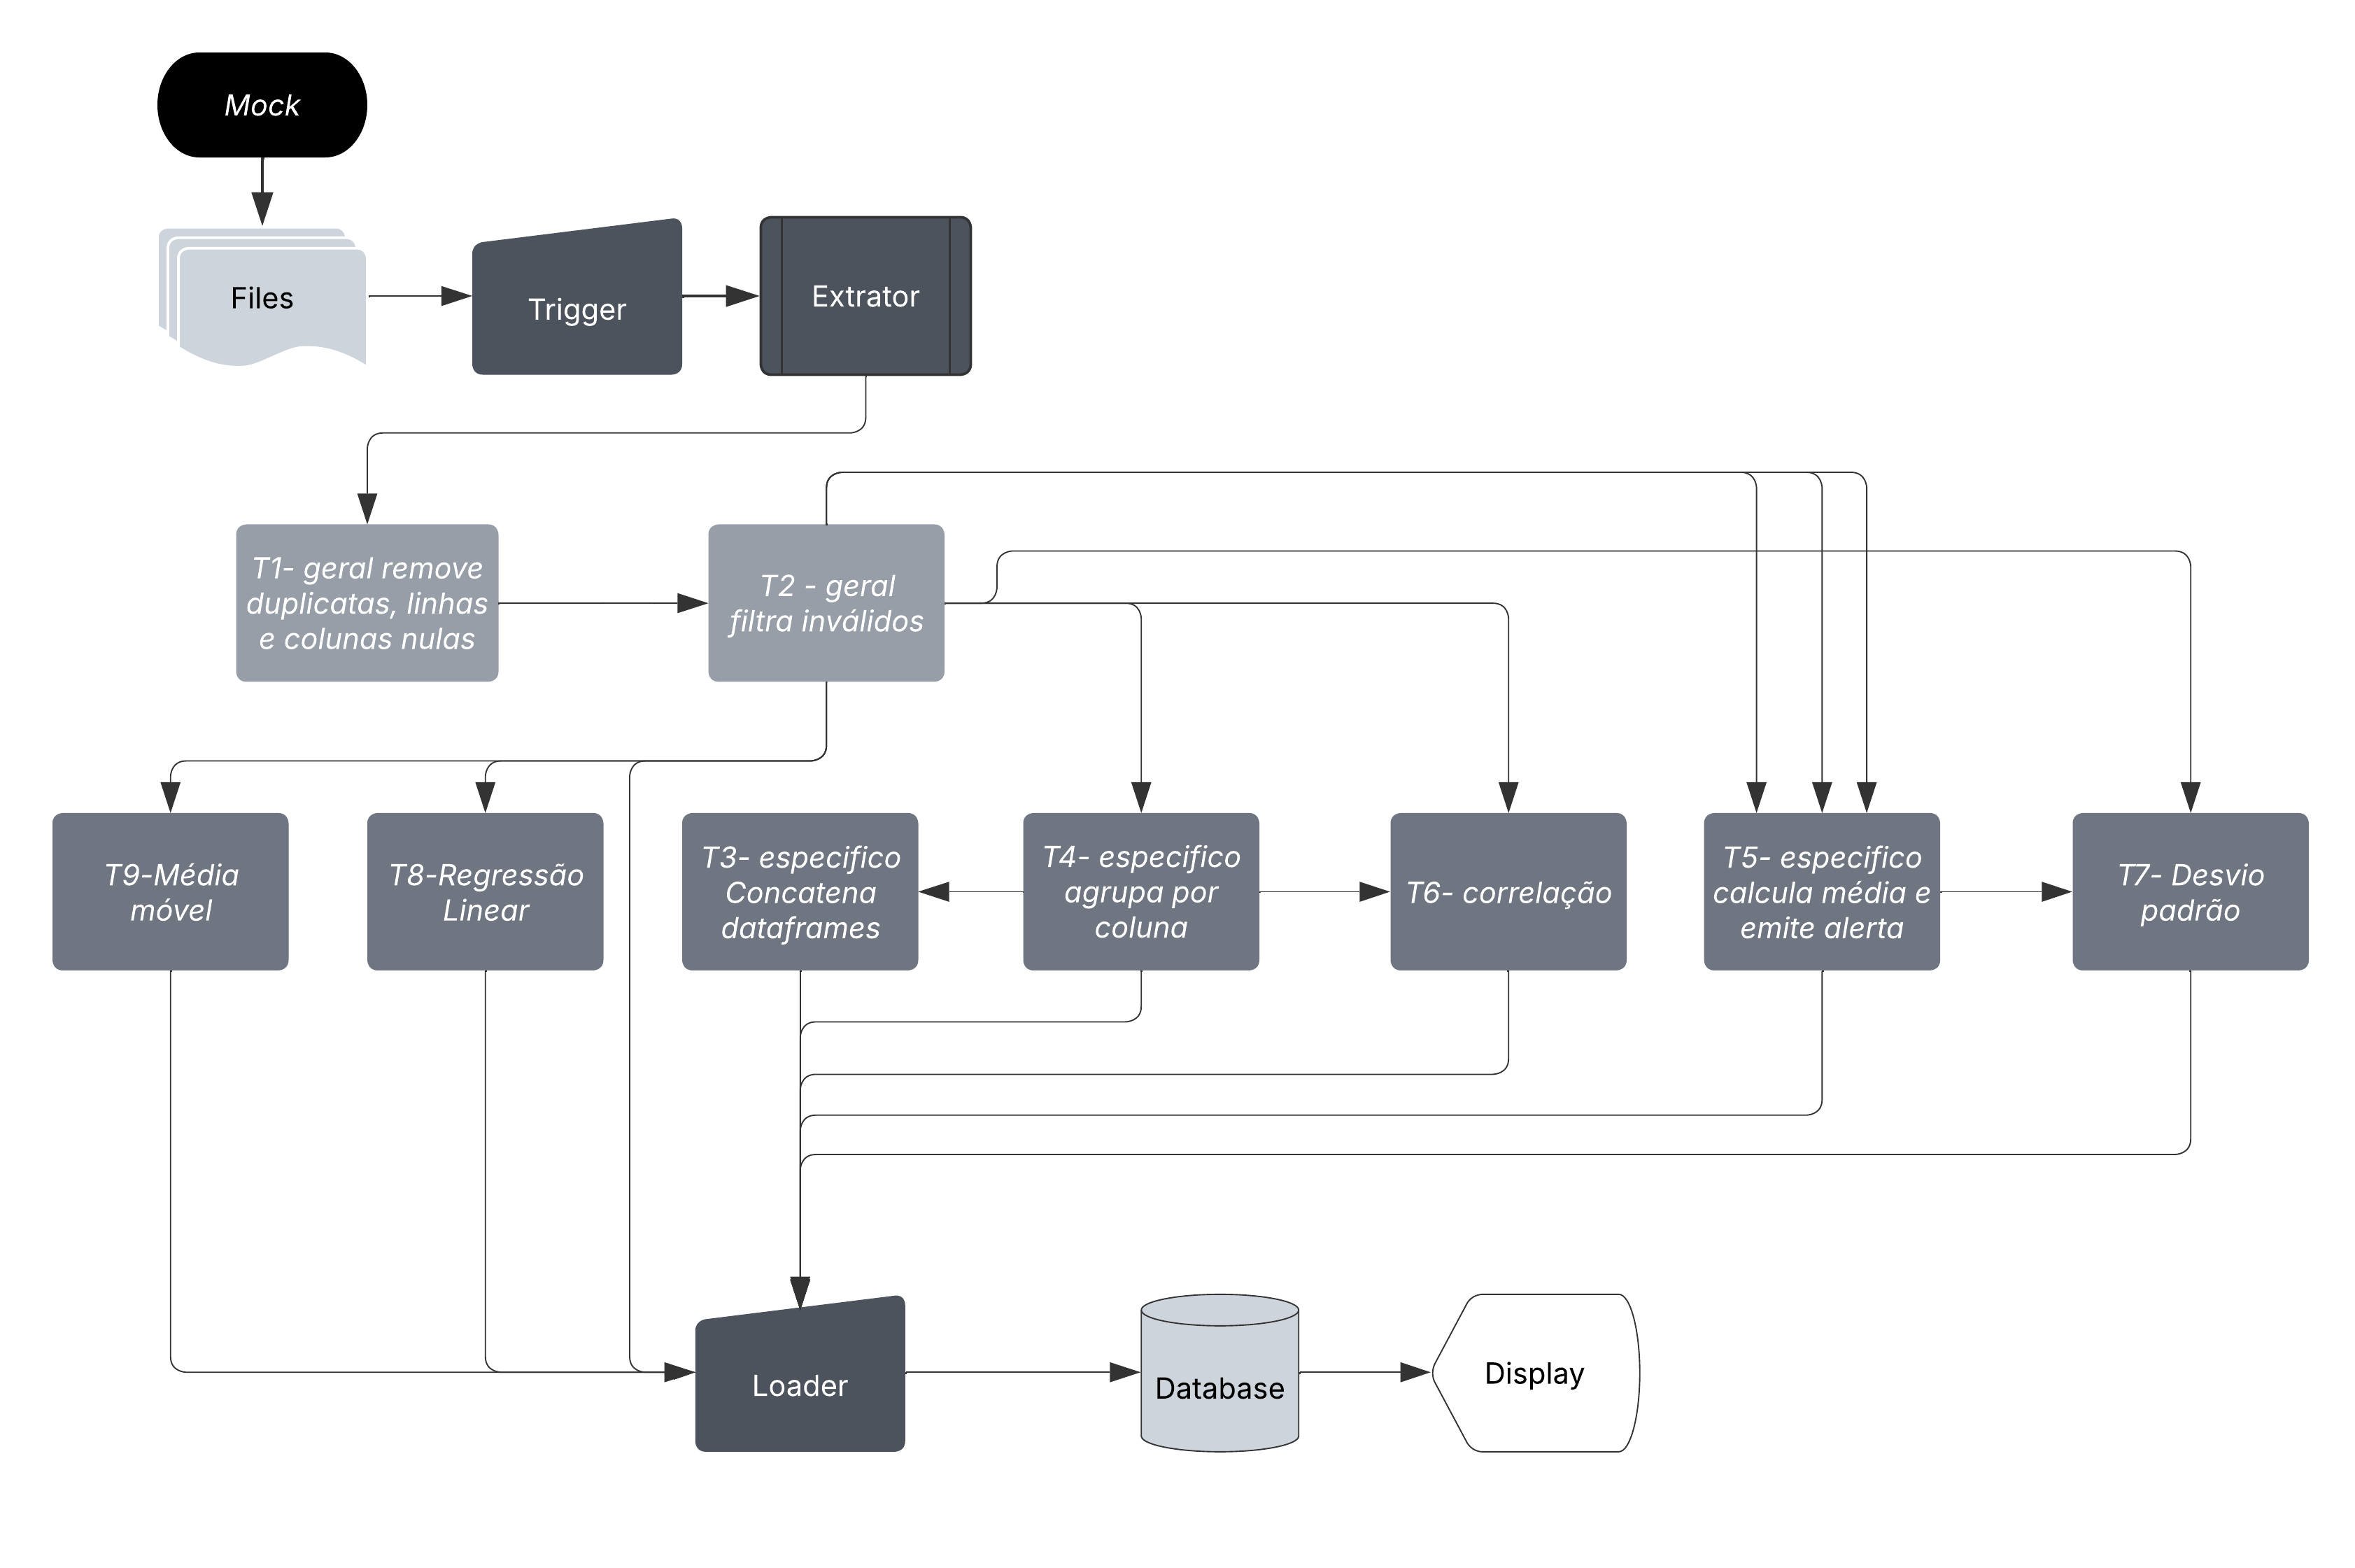
\includegraphics[width=1.1\linewidth]{Fluxograma-A2.png}
    \caption{Fluxograma completo do pipeline de dados}
    \label{fig:pipeline}
\end{figure}

\subsection*{Exemplos na prática}

\subsubsection*{Pontos fortes da abordagem}

\subsubsection*{Pontos fracos da abordagem}




\section{Análise de tempo de execução}



\section{Manual de Execução do Pipeline local}

Esta seção descreve os passos necessários para compilar, implantar e executar todo o pipeline de processamento de dados utilizando Docker e Docker Compose.

\subsection*{Pré-requisitos}

Antes de iniciar, certifique-se de que os seguintes softwares estejam instalados no sistema:

\begin{itemize}
    \item \textbf{Docker}: Ambiente de contêineres para isolamento e portabilidade.
    \item \textbf{Docker Compose}: Orquestração de múltiplos contêineres via arquivo \texttt{docker-compose.yml}
    % \item \textbf{Make} (opcional): para facilitar a execução de comandos com um \texttt{Makefile}.
\end{itemize}

\subsection*{Etapas para Compilar e Executar o Projeto}

\begin{enumerate}
    \item \textbf{Clone o repositório do projeto:}
    \begin{verbatim}
    git clone https://github.com/PAULA-123/ScalableComputingA2
    cd ScalableComputingA2

    ou baixe o projeto completo zip
    \end{verbatim}

    \item \textbf{Compile e suba os serviços com Docker Compose:}
    \begin{verbatim}
    docker-compose up --build
    \end{verbatim}

    Este comando compila as imagens necessárias e inicia os contêineres do Kafka, mock generator, tratadores, API e dashboard.

    \item \textbf{Verifique o status dos serviços:}
    \begin{verbatim}
    docker-compose ps
    \end{verbatim}

    \item \textbf{Acesse o dashboard de visualização:}

    Após a inicialização, o dashboard Streamlit estará disponível em:
    \begin{verbatim}
    http://localhost:8501
    \end{verbatim}

    \item \textbf{Acesse a API intermediária (FastAPI):}

    A documentação automática da API pode ser acessada via:
    \begin{verbatim}
    http://localhost:8000/docs
    \end{verbatim}

    \item \textbf{Interromper os serviços:}
    \begin{verbatim}
    docker-compose down
    \end{verbatim}

    Este comando encerra todos os contêineres e libera os recursos utilizados.

    \item \textbf{(Opcional) Limpeza de volumes e imagens:}
    \begin{verbatim}
    docker system prune -a
    docker volume prune
    \end{verbatim}
    Use com cautela — isso removerá todas as imagens e volumes não utilizados.
\end{enumerate}

\subsection*{Observações Adicionais}

\begin{itemize}
    \item O serviço de mock (\texttt{mock-generator}) gera dados sintéticos e envia para os tópicos Kafka automaticamente.
    \item Os tratadores Spark são iniciados automaticamente e consomem os dados assim que os tópicos estão disponíveis.
    \item O pipeline é tolerante a falhas e reinicia os contêineres automaticamente em caso de quedas.
\end{itemize}



\section{Manual de Execução do Pipeline Nuvem}

\end{document}
